\documentclass{beamer}

\usepackage[utf8]{inputenc}
\usepackage{default}
\usepackage{ulem}
\usepackage{graphicx, subfig}

\setbeamertemplate{navigation symbols}{}

\usetheme{Ilmenau}
\setbeamercolor{frametitle}{fg=black,bg=white}
\setbeamercolor{title}{fg=black,bg=red!75!black}

\newcommand{\OP}[1]{{\bf\widehat{#1}}}

\beamersetuncovermixins{\opaqueness<1>{25}}{\opaqueness<2->{15}}
\begin{document}
\title{The basics of the DMC code}
\author{Jørgen Høgberget}
\date{} 

\begin{frame}
\titlepage
\end{frame}

\begin{frame}\frametitle{Table of contents}\tableofcontents
\end{frame} 


\section{Aims and limitations} 
\subsection{Introduction}

\begin{frame}\frametitle{What can it do?} 

\begin{alertblock}{Quantities of interest}
\begin{itemize}
 \item Ground state energies and densities.
 \item Energy distributions.
\end{itemize}
\end{alertblock}

\pause
\begin{alertblock}{Implemented Systems}
\begin{itemize}
\item Harmonic oscillator systems (2D, 3D, doublewells)
\item Atomic systems (Atoms, homonuclear diatomic molecules)
\end{itemize}
\end{alertblock}

\end{frame}

\begin{frame}\frametitle{Underlying goals and assumptions}

\begin{alertblock}{In a nutshell}
 \textit{Ab-initio}, Efficiency, Transparency
\end{alertblock}

\pause

\begin{alertblock}{Specifics: Assumptions}
\begin{itemize}
 \item Single Slater-determinant ansatz.
 \item Single-parameter Jastrow correlation function.
\end{itemize}
\end{alertblock}

\end{frame}


\begin{frame}\frametitle{Why ab-initio?}

\begin{itemize}
 \item Avoid self-consistency in multi-scale modelling.
 \pause\item System acts independent of our aims of the computation - nature is not influenced by our intentions.
 \pause\item Fundamental modelling: High academic eigenvalue.
 \pause\item Downside: It is harder to solve equations when you cannot assume to know the answer (even if you do).
\end{itemize}

\end{frame}

\begin{frame}\frametitle{Efficiency vs. generalization and precision}

The precision of DMC (given a model Hamiltonian) is, to first approximation, limited by one thing: \textbf{The trial wave function}.

\pause
\vspace{0.5cm}
General MB. WF. construction:

\begin{equation*}
 \text{SP-basis} \quad \to \quad \text{Det. Basis} \quad \to \quad \text{Combine Determinants}
\end{equation*}


\end{frame}

\begin{frame}\frametitle{Efficiency vs. generalization and precision}

The precision of QMC (given a model Hamiltonian) is, to first approximation, limited by one thing: \textbf{The trial wave function}.


\vspace{0.5cm}
Compromise to ensure efficiency and ``ideal scaling``

\begin{equation*}
 \text{SP-basis} \quad \to \quad \text{Det. } \text{\sout{Basis}} \quad \not\to \quad \text{\sout{Combine Determinants}}
\end{equation*}


\end{frame}

\section{The Code: Transparency is win}
\subsection{Describing a system}

\begin{frame}[containsverbatim]\frametitle{Start from the bottom up}
 
 \begin{itemize}
    \item Implement single particle wave functions $\Phi_j(\vec r_i)$.
 \end{itemize}

 
\scriptsize
 \begin{verbatim}
class BasisFunctions {
public:
    BasisFunctions();
    
    virtual double eval(const Walker* walker, int i) = 0;
};
 \end{verbatim}
\normalsize

\end{frame}


 
\scriptsize
\begin{frame}[containsverbatim]
 \begin{verbatim}
//n_x = n_y = n_z = 1
double HarmonicOscillator3D_15::eval(const Walker* walker, int i) {

    x = walker->r(i, 0);
    y = walker->r(i, 1);
    z = walker->r(i, 2);
    
    //x*y*z*exp(-k^2*r^2/2)
    
    H = x*y*z;
    return H*(*exp_factor);
    
}
 \end{verbatim}
\end{frame}
\normalsize


\begin{frame}

 \begin{itemize}
    \item Implement single particle wave functions $\Phi_j(\vec r_i)$.
    \item Extensive bases should be generated with the supplied \textit{SymPy}-script (read Appendix C in the Thesis).
    \pause \item Setup the determinant.
\end{itemize}

\end{frame}

\begin{frame}[containsverbatim]
\scriptsize
 \begin{verbatim}
class Orbitals {
protected:

    BasisFunctions** basis_functions; 
    BasisFunctions*** del_basis_functions;
    BasisFunctions** lapl_basis_functions; 

    //Important: All basis elements and the orbital wrapper 
    //SHARE parameter references
    virtual void set_parameter(double parameter, int n) = 0;

public:

    Orbitals(int n_p, int dim);

    virtual double      phi(const Walker* walker, int i, int q);
    virtual double  del_phi(const Walker* walker, int i, int q, int d);
    virtual double lapl_phi(const Walker* walker, int i, int q);

};
 \end{verbatim}
\normalsize
\end{frame}


\begin{frame}[containsverbatim]
\scriptsize
 \begin{verbatim}
double Orbitals::phi(const Walker* walker, int particle, int q_num) {
    return basis_functions[q_num]->eval(walker, particle);
}

double Orbitals::del_phi(const Walker* walker, int particle, int q_num, int d) {
    return del_basis_functions[d][q_num]->eval(walker, particle);
}

double Orbitals::lapl_phi(const Walker* walker, int particle, int q_num) {
    return lapl_basis_functions[q_num]->eval(walker, particle);
}
 \end{verbatim}
\normalsize

Idea: Fill the basis function vectors in the subclass constructor, and you're good to go.

\end{frame}

\begin{frame}[containsverbatim]
\scriptsize
 \begin{verbatim}
HaromonicOscillator::HarmonicOscillator{
    ...

    basis_functions[0] = new HarmonicOscillator3D_0(...);
    basis_functions[1] = new HarmonicOscillator3D_1(...);
    basis_functions[2] = new HarmonicOscillator3D_2(...);
    ...

    dell_basis_functions[0][0] = new dell_HarmonicOscillator3D_0_x(...);
    dell_basis_functions[1][0] = new dell_HarmonicOscillator3D_0_y(...);
    dell_basis_functions[2][0] = new dell_HarmonicOscillator3D_0_z(...);
    dell_basis_functions[0][1] = new dell_HarmonicOscillator3D_1_x(...);
    dell_basis_functions[1][1] = new dell_HarmonicOscillator3D_1_y(...);
    dell_basis_functions[2][1] = new dell_HarmonicOscillator3D_1_z(...);
    ...

    lapl_basis_functions[0] = new lapl_HarmonicOscillator3D_0(...);
    lapl_basis_functions[1] = new lapl_HarmonicOscillator3D_1(...);
    ...
    
}
 \end{verbatim}
\normalsize
 
\end{frame}

\begin{frame}

 \begin{itemize}
    \item Implement single particle wave functions $\Phi_j(\vec r_i)$.
    \item Extensive bases should be generated with the supplied \textit{SymPy} script (read Appendix C in the Thesis).
    \item Setup the determinant.
    \item Luckily this is done automatically by the SymPy script.. Such a manual coding opens up possibility for seting up \textit{any} of the determinants, not just the ''ground state``.
\end{itemize}

\pause

Overcomplicated?

\pause 

Perhaps it can be simplified? Doesn't matter really. This way of structuring makes implementations of expanded \textbf{SP} bases and molecules trivial.

\end{frame}

\begin{frame}[containsverbatim]\frametitle{Expanded Bases}
\scriptsize
\begin{verbatim}
class ExpandedBasis : public Orbitals {
public:
    ExpandedBasis(...);

    double phi(...);
    double del_phi(...);
    double lapl_phi(...);
    
protected:
    arma::mat coeffs;

    Orbitals* basis;

};
\end{verbatim}
\normalsize
\end{frame}


\begin{frame}[containsverbatim]\frametitle{Expanded Bases}
\scriptsize
\begin{verbatim}
double ExpandedBasis::phi(const Walker* walker, int i, int q) {

    double value = 0;

    //Dividing basis_size by half assuming a two-level system.
    for (int m = 0; m < basis_size / 2; m++) {
        value += coeffs(q, m) * basis->phi(walker, i, m);
    }

    return value;

}
\end{verbatim}
\normalsize

Can be loaded into the QMC machinery as any other Orbital instance.
\end{frame}




\begin{frame}
\begin{center}
 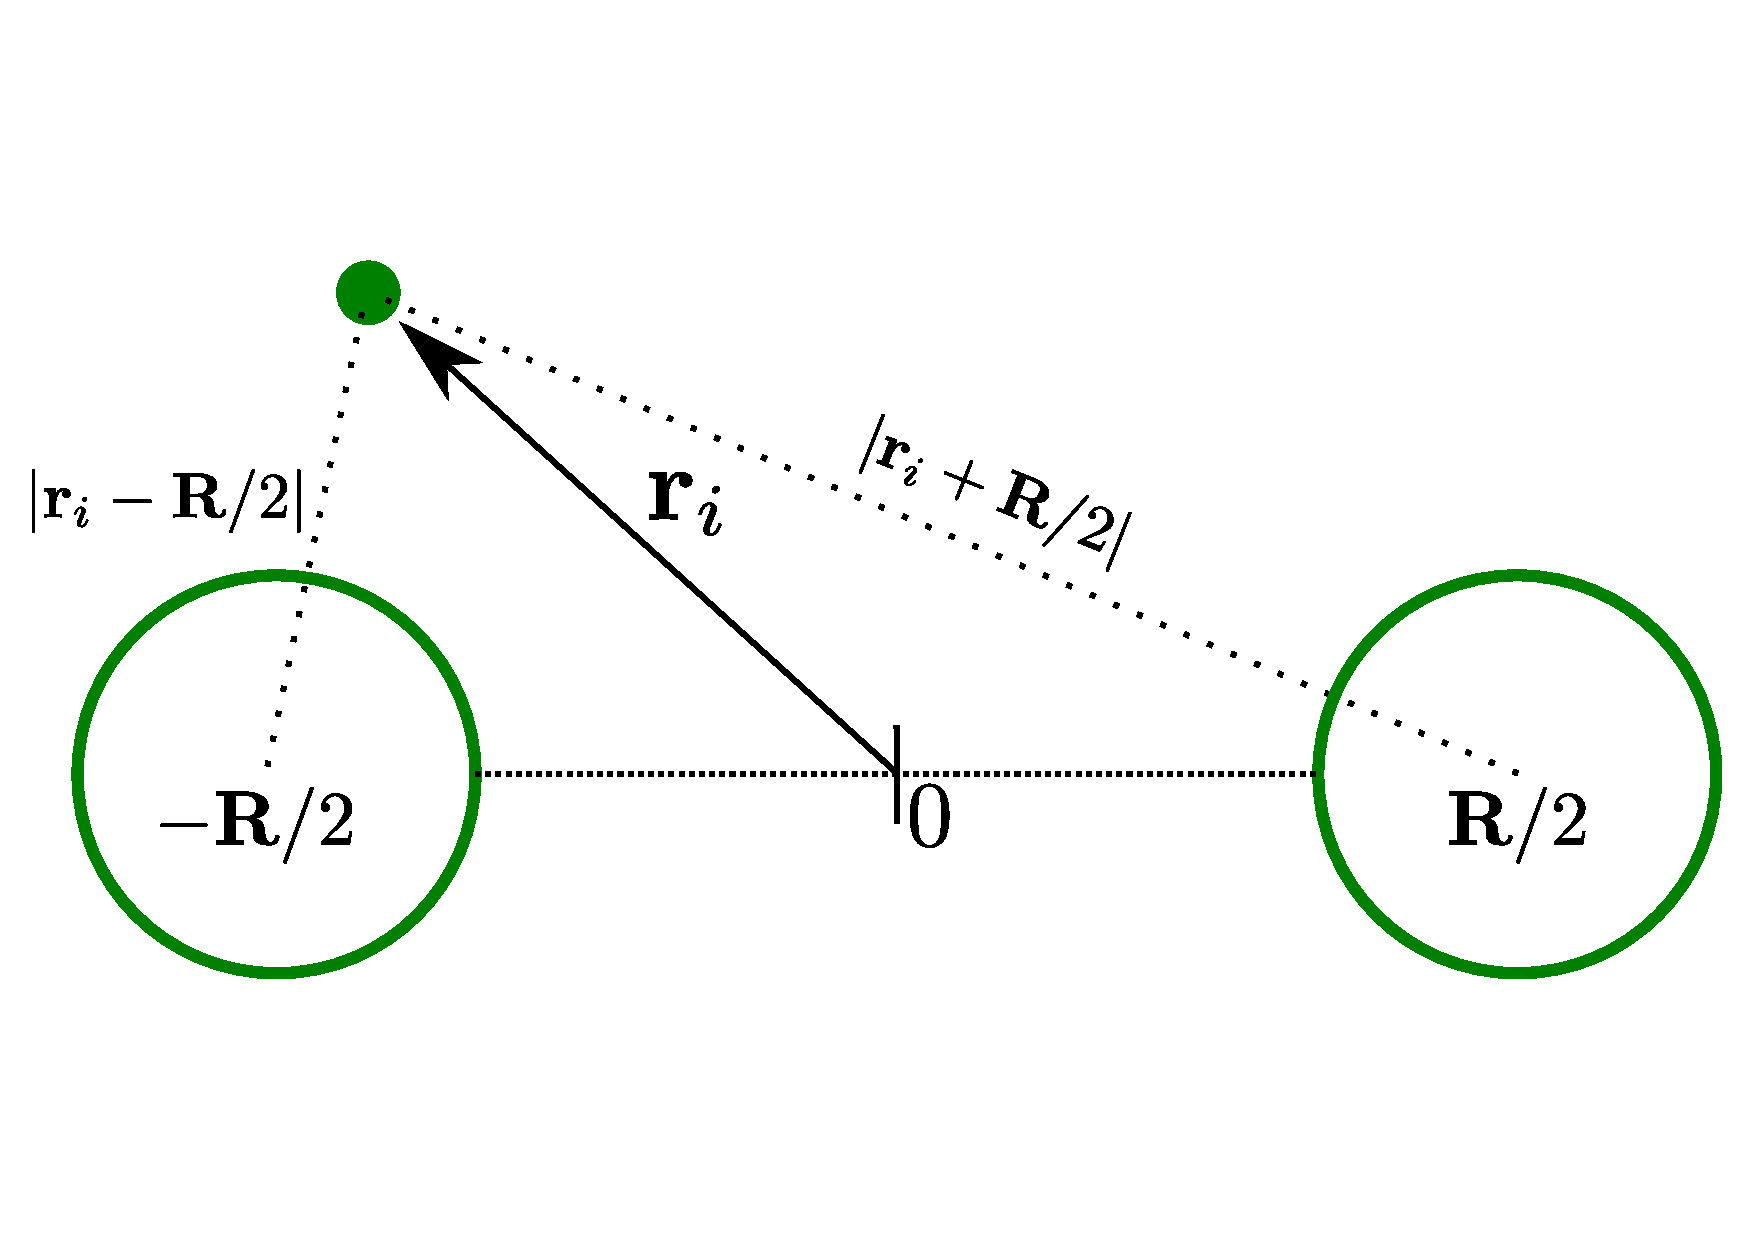
\includegraphics[scale=0.35]{Molecules.pdf}
\end{center}
\end{frame}



\begin{frame}\frametitle{(di)Molecules}
 \begin{equation*}
 \OP{H}_{\mathrm{Mol.}}(\mathbf{r}, \mathbf{R}) = \sum_{i=1}^N \left[-\frac{1}{2}\nabla_i^2 - \frac{Z}{|\mathbf{r}_i + \mathbf{R}/2|} - \frac{Z}{|\mathbf{r}_i - \mathbf{R}/2|}\right] + \frac{Z^2}{R} + \sum_{i<j} \frac{1}{r_{ij}}.
\end{equation*}
\end{frame}


\begin{frame}[containsverbatim]\frametitle{(di)Molecules}
\scriptsize
\begin{verbatim}
double DiAtomCore::get_pot_E(const Walker* walker) const {
    
    double e_pot = 0;
    double com_corr, shared;
    
    double quarterR2 = 0.25*(*R)*(*R);
    for (int i = 0; i < n_p; i++) {
        
        shared = walker->get_r_i2(i)+ quarterR2;
        com_corr = (*R)*walker->r(i, 0);
        
        e_pot -= Z*(1./sqrt(shared + com_corr) + 1./sqrt(shared - com_corr));
    }

    e_pot += Z*Z/(*R);
    
    return e_pot;
    
}
\end{verbatim}
\normalsize
\end{frame}


\begin{frame}[containsverbatim]\frametitle{(di)Molecules}
\scriptsize
\begin{verbatim}
class DiTransform : public Orbitals {
...

protected:
    double* R;

    Orbitals* nucleus1, nucleus2;
    Walker* walker_nucleus1, walker_nucleus2;

    //Wrap wrap wrap, it's christmas!
    double get_parameter(int n) {
        return nucleus1->get_parameter(n);
    }

    void set_parameter(double parameter, int n) {
        nucleus1->set_parameter(parameter, n);
        nucleus2->set_parameter(parameter, n);
    }
};
\end{verbatim}
\normalsize
\end{frame}

\begin{frame}\frametitle{(di)Molecules}
\begin{itemize}
 \item A Walker instance for each nucleus ensures minimal overhead when transforming from atoms to molecules (precalculates distances etc.). \pause
 \item An Orbital instance for each nucleus ensures that all optimizations from the single atom scheme can be carried to the molecular one (precalculates exponential factors etc.). \pause
 \item QMC is not memory intensive. Matrices are of size $N \times N$ at max, where $N=100$ is the world record.
\end{itemize}

\end{frame}



\begin{frame}[containsverbatim]\frametitle{(di)Molecules}
\scriptsize
\begin{verbatim}
void DiTransform::set_qnum_indie_terms(Walker* walker, int i) {

    walker->calc_r_i(i);

    //Apply the molecular transformation!
    walker_nucleus1->r.row(i) = walker->r.row(i);
    walker_nucleus2->r.row(i) = walker->r.row(i);

    walker_nucleus1->r(i, 0) += (*R) / 2;
    walker_nucleus2->r(i, 0) -= (*R) / 2;

    double shared = walker->get_r_i2(i) + 0.25 * (*R)*(*R);
    double comm_spec = walker->r(i, 0)*(*R);

    walker_nucleus1->r2(i) = shared + comm_spec;
    walker_nucleus2->r2(i) = shared - comm_spec;

    nucleus1->set_qnum_indie_terms(walker_nucleus1, i);
    nucleus2->set_qnum_indie_terms(walker_nucleus2, i);

}
\end{verbatim}
\normalsize
\end{frame}
\begin{frame}\frametitle{Transforming SPWFs to molecular SPWFs}

Plus and minus refers to the two nuclei, $H$ refers to the standard hydrogen-like basis.

\begin{align}
 \phi_{nlm}^+ (\mathbf{r}_i, \mathbf{R}) &= \phi_{nlm}^\mathrm{H}(\mathbf{r}_i + \mathbf{R}/2) + \phi_{nlm}^\mathrm{H}(\mathbf{r}_i - \mathbf{R}/2)\label{eq:moleculeTransPlus},\notag \\
 \phi_{nlm}^- (\mathbf{r}_i, \mathbf{R}) &= \phi_{nlm}^\mathrm{H}(\mathbf{r}_i + \mathbf{R}/2) - \phi_{nlm}^\mathrm{H}(\mathbf{r}_i - \mathbf{R}/2)\label{eq:moleculeTransMin},\notag
\end{align}

which reads ``electron surrounding first nucleus combined with electron surrounding second nucleus''.

\end{frame}

\begin{frame}[containsverbatim]\frametitle{Applying the transformation}
\scriptsize
\begin{verbatim}
double DiTransform::phi(const Walker* walker, int i, int q) {

    (void) walker;
    int sign = minusPower(q);

    return nucleus1->phi(walker_nucleus1, i, q / 2) +
            sign * nucleus2->phi(walker_nucleus2, i, q / 2);
            
}
\end{verbatim}
\normalsize
\end{frame}

\begin{frame}\frametitle{We can reuse closed form expressions}
 \begin{align}
 \mathbf{j}\cdot \nabla_i \phi_{nlm}^\pm (\mathbf{r}_i, \mathbf{R}) &= \underbrace{\frac{\partial (y_i + R_y/2)}{\partial y_i}}_{1}\frac{\partial \phi_{nlm}^\mathrm{H}(\mathbf{r}_i + \mathbf{R}/2)}{\partial (y_i + R_y/2)} \notag \\
  &\pm \underbrace{\frac{\partial (y_i - R_y/2)}{\partial y_i}}_{1}\frac{\partial \phi_{nlm}^\mathrm{H}(\mathbf{r}_i - \mathbf{R}/2)}{\partial (y_i - R_y/2)} \notag\\
  &= \frac{\partial \phi_{nlm}^\mathrm{H}(\mathbf{r}_i + \mathbf{R}/2)}{\partial (y_i + R_y/2)} \pm \frac{\partial \phi_{nlm}^\mathrm{H}(\mathbf{r}_i - \mathbf{R}/2)}{\partial (y_i - R_y/2)} \notag\\
  &=  \frac{\partial \phi_{nlm}^\mathrm{H}(\mathbf{\tilde R_i^+})}{\partial \tilde Y_i^+} \pm \frac{\partial \phi_{nlm}^\mathrm{H}(\mathbf{\tilde R_i^-})}{\partial \tilde Y_i^-}, \label{eq:MoleculeWorksWithOldFunctions} \notag
\end{align}
\end{frame}

\begin{frame}[containsverbatim]\frametitle{We can reuse closed form expressions}
\scriptsize
\begin{verbatim}
double DiTransform::lapl_phi(const Walker* walker, int particle, int q_num) {

    (void) walker;
    int sign = minusPower(q_num);

    return nucleus1->lapl_phi(walker_nucleus1, particle, q_num / 2) +
            sign * nucleus2->lapl_phi(walker_nucleus2, particle, q_num / 2);
}
\end{verbatim}
\normalsize
\end{frame}

\begin{frame}\frametitle{Generalizable to N-atomic molecules?}
 
 \textbf{YES.}\pause
 \vspace{0.5cm}
 
 Challenges:
 \begin{itemize}
  \item Current model breaks down around $\mathrm{O}_2$.
  \item Need a better trial wave function.
  \item Multi-determinants are out of the question.
  \item More advanced Jastrow is out of the question.
  \item Expanded single particle states are gold.
  \item Slater orbitals are gold.
 \end{itemize}

 
 
 
\end{frame}


\scriptsize
\begin{frame}
\begin{table}
\begin{center}
\begin{tabular}{lrccrlrr}
Molecule & $R$ & & \qquad & $E_\mathrm{VMC}$ & & \qquad $E_\mathrm{DMC}$ & \qquad\,\, Expt. \\
\hline\hline
\ \\
$\mathrm{H_2}$ & 1.4   & &\qquad & -1.1551(3)    & \qquad   & -1.1745(3)   & \qquad $-1.1746$   \\
\ \\
\vdots & & & & & & & \\
\ \\
$\mathrm{O_2}$ & 2.282 & &\qquad & -143.97(2)    & \qquad   & -148.53(2)   & \qquad $-150.3268$  \\
\ \\
\end{tabular}
\caption{Refs. for $R$ and Expt.: \cite{H_He_exact, UmrigarMolecules, ExactMolecules}.}
\label{tab:MoleculesRes}
\end{center}
\end{table}
\end{frame}
\normalsize



\begin{frame}\frametitle{Parametrizations}
 \begin{figure}
 \begin{center}
  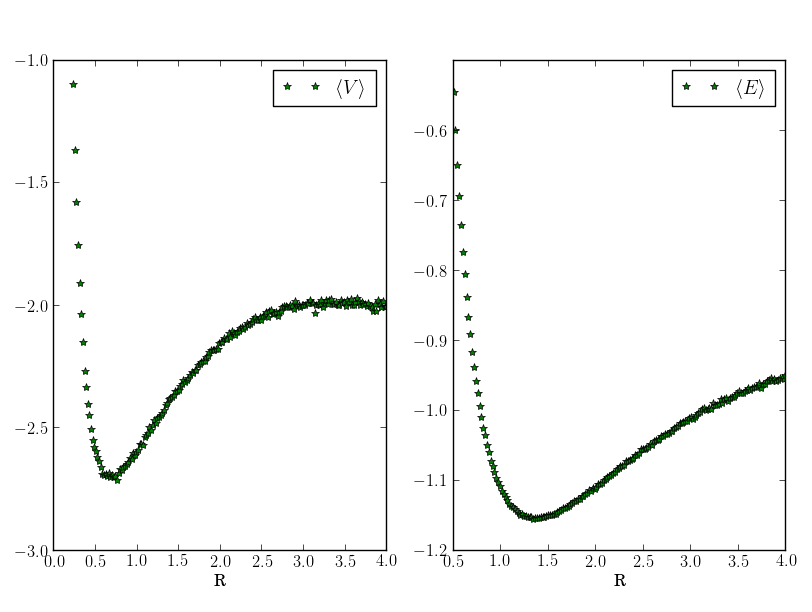
\includegraphics[scale=0.35]{R_vs_E_hyd_pure.png}
  \caption{$\mathrm{H_2}$}
 \end{center}
\end{figure}
\end{frame}


\begin{frame}\frametitle{Parametrizations}
 \begin{figure}
 \begin{center}
  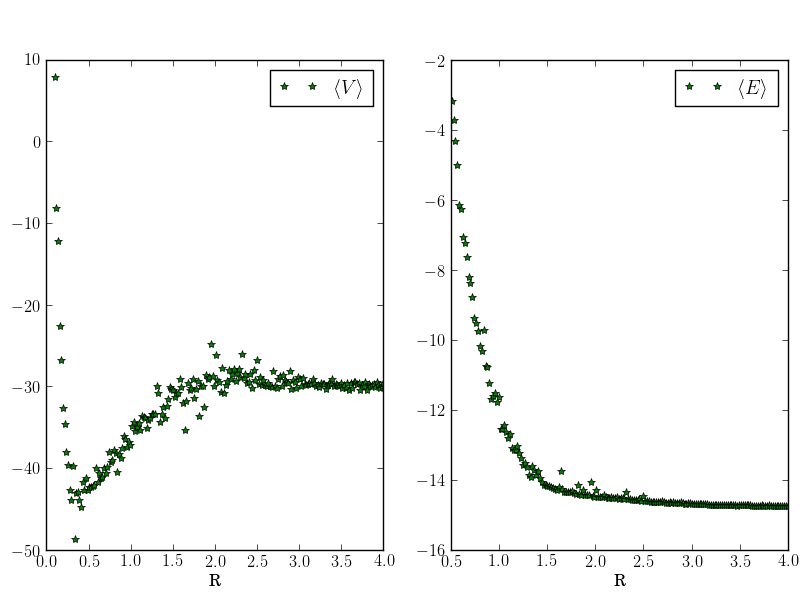
\includegraphics[scale=0.35]{R_vs_E_lit_pure.png}
  \caption{$\mathrm{Li_2}$}
 \end{center}
\end{figure}
\end{frame}


\subsection*{}

\begin{frame}
 \bibliographystyle{plain}
 \bibliography{bibtex}
\end{frame}


\end{document}